% This is the preamble of a LaTeX source code.
\documentclass[10pt,a4paper]{article}

\usepackage{tikz}                % Creating graphics

% Needed for busy beaver Turing machine, see
% https://mirror.dogado.de/tex-archive/graphics/pgf/base/doc/pgfmanual.pd
% p. 102
\usetikzlibrary {arrows.meta, automata, positioning, shadows}

% Color list:
\definecolor{amber}{rgb}{1.0, 0.75, 0.0}
\definecolor{amber(sae/ece)}{rgb}{1.0, 0.49, 0.0}
\definecolor{americanrose}{rgb}{1.0, 0.01, 0.24}
\definecolor{amethyst}{rgb}{0.6, 0.4, 0.8}
\definecolor{applegreen}{rgb}{0.55, 0.71, 0.0}
\definecolor{armygreen}{rgb}{0.29, 0.33, 0.13}
\definecolor{coquelicot}{rgb}{1.0, 0.22, 0.0}
\definecolor{english}{rgb}{0.0, 0.5, 0.0}


\begin{document}

\section {Archetype}

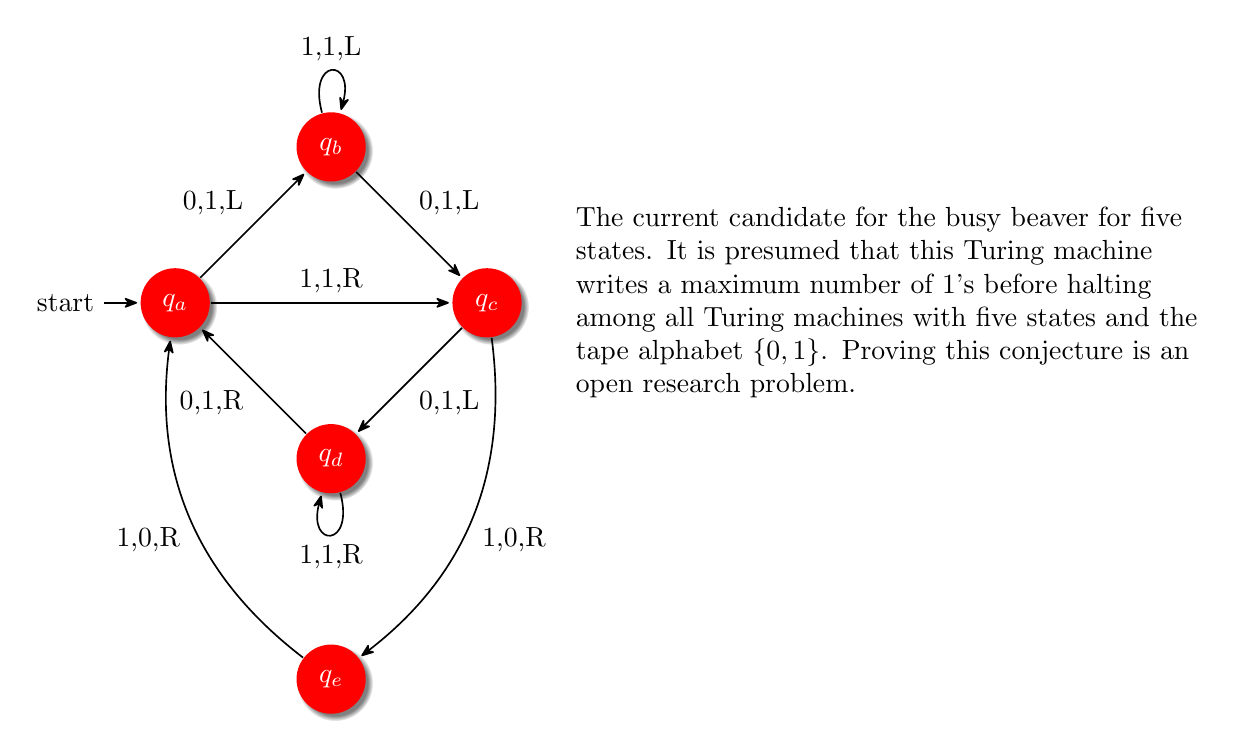
\begin{tikzpicture}[->,>={Stealth[round]},shorten >=1pt,auto,node distance=2.8cm,on grid,semithick,
every state/.style={fill=red,draw=none,circular drop shadow,text=white}]
\node[initial,state] (A) {$q_a$};
\node[state] (B) [above right=of A] {$q_b$};
\node[state] (D) [below right=of A] {$q_d$};
\node[state] (C) [below right=of B] {$q_c$};
\node[state] (E) [below=of D] {$q_e$};
\path (A) edge node {0,1,L} (B)
edge node {1,1,R} (C)
(B) edge [loop above] node {1,1,L} (B)
edge node {0,1,L} (C)
(C) edge node {0,1,L} (D)
edge [bend left] node {1,0,R} (E)
(D) edge [loop below] node {1,1,R} (D)
edge node {0,1,R} (A)
(E) edge [bend left] node {1,0,R} (A);
\node [right=1cm,text width=8cm] at (C)
{
The current candidate for the busy beaver for five states. It is
presumed that this Turing machine writes a maximum number of
$1$'s before halting among all Turing machines with five states
and the tape alphabet $\{0, 1\}$. Proving this conjecture is an
open research problem.
};
\end{tikzpicture}


\section {Playing}

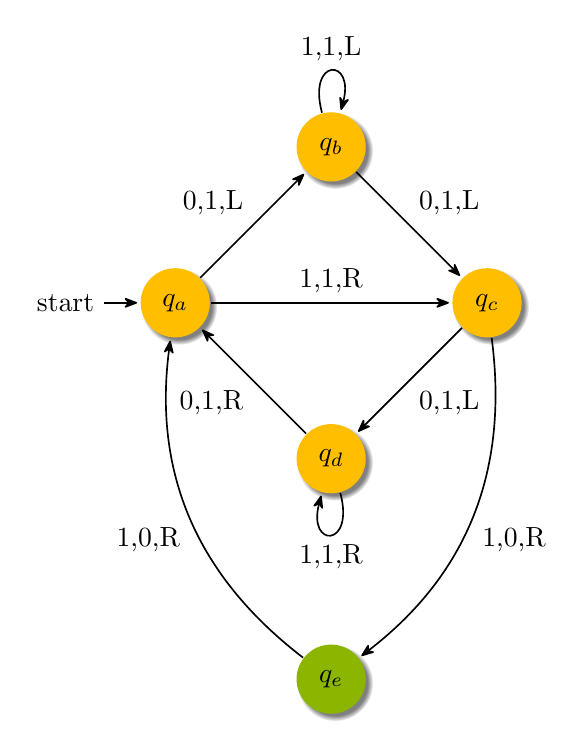
\begin{tikzpicture}[%
    ->,
    >= { Stealth[round] },
    shorten >= 1pt,
    auto,
    node distance = 2.8cm,
    on grid,
    semithick,
    every state/.style = {%
      fill = amber,
      draw = none,
      circular drop shadow,
      text = black }    
  ]
  
\node[initial,state] (A) {$q_a$};
\node[state] (B) [above right=of A] {$q_b$};
\node[state] (D) [below right=of A] {$q_d$};
\node[state] (C) [below right=of B] {$q_c$};
\node[state] (E) [below=of D, fill=applegreen] {$q_e$};

\path
(A) edge node {0,1,L} (B)
edge node {1,1,R} (C)

(B) edge [loop above] node {1,1,L} (B)
edge node {0,1,L} (C)

(C) edge node {0,1,L} (D)
edge [bend left] node {1,0,R} (E)

(D) edge [loop below] node {1,1,R} (D)
edge node {0,1,R} (A)

(E) edge [bend left] node {1,0,R} (A);

\end{tikzpicture}


\section {Preliminary}

\begin{verbatim}
Reference:
https://de.wikipedia.org/wiki/Turingmaschine
https://en.wikipedia.org/wiki/Turing_machine
\end{verbatim}

\begin{description}
  
\item[Beobachtung:]
In der Berufsschule verwendet man bunte Begriffe, die man
2-dimensionalen mit z.T. bidrektionen Pfeilen verbindet und
zwar unspezifiert.

\item[Idee:]
Das ist ein Algorithmus und ein Automat.
Als Modell verwende ich deterministische Turing Maschine,
damit es nicht zu kompliziert wird.

\item[Spiel:]
Jeder Mensch, Mathematiker oder Philosoph spielt dauernd mit irgendwelchen Zeichen:

\item[xxx: ]
Um alles zu vereinfachen, beschränke ich mich auf eine
deterministische Turing Maschine - DTM - oder einen Computer, der das macht,
was - tbd. - er laut Beschreibung kann und zwar sofort - tbd. - ein Ergebnis
sofort liefert, das mit der Erwartiung übereinstimmt.

\item[xxx: ]
Ziemlich frei habe ich alles umdefininiert:

DTM = (C, I, R, B, F, T, S)
\end{description}
  
\begin{description}
\item[C := ] States of the computer
\item[I := ] I/O characters (abstract)
\item[M := ] Memory
\item[B := ] Power on or boot phase
\item[F := ] Functions
\item[T := ] Timeout actions like powersaveing
\item[S := ] Power off or shutdown
\end{description}

\vskip 20pt

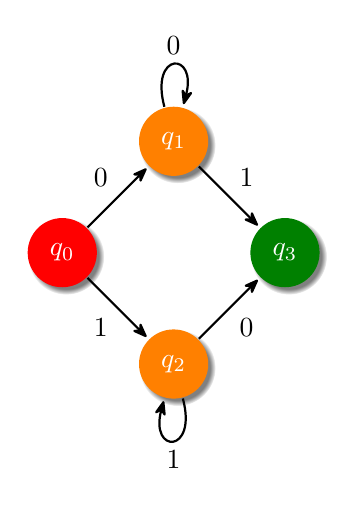
\begin{tikzpicture} [%
    shorten >= 1pt,
    node distance = 2cm,
    on grid,
    >= {Stealth[round]},
    thick,    
    every state/.style = {%
      fill,draw = none,orange,
      text = white,
      circular drop shadow },    
    accepting/.style ={%
      green!50!black,
      text = white },    
    initial/.style ={%
      red, text = white}
  ]
  
\node[state,initial]    (q_0) {$q_0$};
\node[state]            (q_1) [above right=of q_0] {$q_1$};
\node[state]            (q_2) [below right=of q_0] {$q_2$};
\node[state,accepting]  (q_3) [below right=of q_1] {$q_3$};

\path[->]
(q_0) edge node [above left] {0} (q_1)
edge node [below left] {1} (q_2)

(q_1) edge node [above right] {1} (q_3)
edge [loop above] node {0} ()

(q_2) edge node [below right] {0} (q_3)
edge [loop below] node {1} ();

\end{tikzpicture}

\section {Derivation}

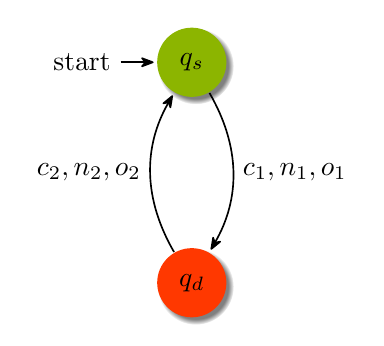
\begin{tikzpicture} [%
    ->,
    >= { Stealth[round] },
    shorten >= 1pt,
    auto,
    node distance = 2.8cm,
    on grid,
    semithick,
    every state/.style = {%
      fill = amber,
      draw = none,
      circular drop shadow,
      text = black }    
  ]

  \node[initial, state, fill=applegreen] (S) {$q_s$};
  \node[state] (D) [below=of S, fill=coquelicot] {$q_d$};

  \path
  (S) edge [bend left] node {$c_1,n_1,o_1$} (D)
  (D) edge [bend left] node {$c_2,n_2,o_2$} (S);
  
\end{tikzpicture}


\vskip 16pt
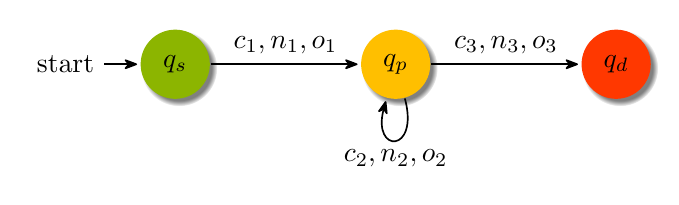
\begin{tikzpicture} [%
    ->,
    >= { Stealth[round] },
    shorten >= 1pt,
    auto,
    node distance = 2.8cm,
    on grid,
    semithick,
    every state/.style = {%
      fill = amber,
      draw = none,
      circular drop shadow,
      text = black }    
  ]

  \node[initial, state, fill=applegreen] (S) {$q_s$};
  \node[state] (P) [right=of S] {$q_p$};
  \node[state] (D) [right=of P, fill=coquelicot] {$q_d$};

  \path
  (S) edge node {$c_1,n_1,o_1$} (P)
  (P) edge [loop below] node {$c_2,n_2,o_2$} (P)
  (P) edge node {$c_3,n_3,o_3$} (D);
  
\end{tikzpicture}



\vskip 16pt
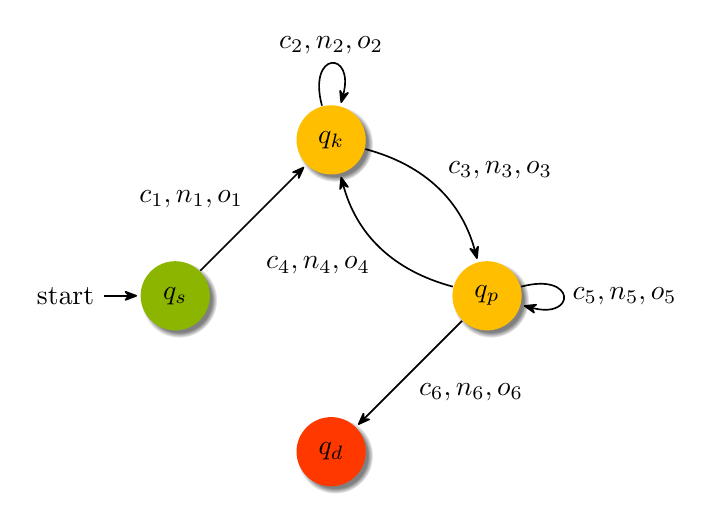
\begin{tikzpicture} [%
    ->,
    >= { Stealth[round] },
    shorten >= 1pt,
    auto,
    node distance = 2.8cm,
    on grid,
    semithick,
    every state/.style = {%
      fill = amber,
      draw = none,
      circular drop shadow,
      text = black }    
  ]

  \node[initial, state, fill=applegreen] (S) {$q_s$};
  \node[state] (K) [above right=of S] {$q_k$};
  \node[state] (P) [below right=of K] {$q_p$};
  \node[state] (D) [below right=of S, fill=coquelicot] {$q_d$};
  
  \path
  (S) edge node {$c_1,n_1,o_1$} (K)
  
  (K) edge [loop above] node {$c_2,n_2,o_2$} (K)
  edge [bend left] node {$c_3,n_3,o_3$} (P)

  (P) edge [bend left] node {$c_4,n_4,o_4$} (K)
  edge [loop right] node {$c_5,n_5,o_5$} (P)

  (P) edge node {$c_6,n_6,o_6$} (D);
  ;
  
\end{tikzpicture}


\begin{verbatim}

Contents

1. Subject - s:     Die Tractatus Dimensionen
                    oder wie alle im Weltall denken
2. Knowledge - k:   Rezitation des Tractatus
3. Proposition - p: Literate Programming / LuaTeX
4. Deadline - p:    23.12.2022
5. Hypothesis - h:  i. Begriffe sind Koordinatenachsen

Legend:
Eine Landkarte versteht man über eine
Übersetzung.
https://de.wikipedia.org/wiki/Legende_(Karte)

Colors:
Wenn man die Ampelfarben nicht versteht,
kann man ganz schnell sterben.

htps://de.wikipedia.org/wiki/Ampel

1. s <-> d

2. s -> l(p) -> d

3.   -> l(k) <-
    |          |
    s          v
              l(p)
               |
           d <-

\end{verbatim}

\end{document}
